\documentclass[border=15pt, multi, tikz]{standalone}
\usepackage{import}
\subimport{./layers/}{init}
\usetikzlibrary{positioning,calc}
\usetikzlibrary{3d} %for including external image 

\def\ConvColor{rgb:yellow,5;red,2.5;white,5}
\def\ConvReluColor{rgb:yellow,5;red,5;white,5}
\def\PoolColor{rgb:red,1;black,0.3}
\def\DcnvColor{rgb:blue,5;green,2.5;white,5}
\def\SoftmaxColor{rgb:magenta,5;black,7}
\def\SumColor{rgb:blue,5;green,15}
\def\MBConvColor{rgb:blue,2;green,5;white,5}

\begin{document}
\begin{tikzpicture}
\tikzstyle{connection}=[ultra thick,every node/.style={sloped,allow upside down},draw=\edgecolor,opacity=0.7]


% Generalized Audio Fine-Tuned EfficientNet B0 Model Architecture
%%%%%%%%%%%%%%%%%%%%%%%%%%%%%%%%%%%%%%%%%%%%%%%%%%%%%%%%%%%%%%%%%%%%%%%%%%%%%%%%%%%%%%%%
%% Draw Layer Blocks
%%%%%%%%%%%%%%%%%%%%%%%%%%%%%%%%%%%%%%%%%%%%%%%%%%%%%%%%%%%%%%%%%%%%%%%%%%%%%%%%%%%%%%%%

% Input waveform layer
\node[canvas is zy plane at x=-3] (waveform) at (-0.5,0,0) {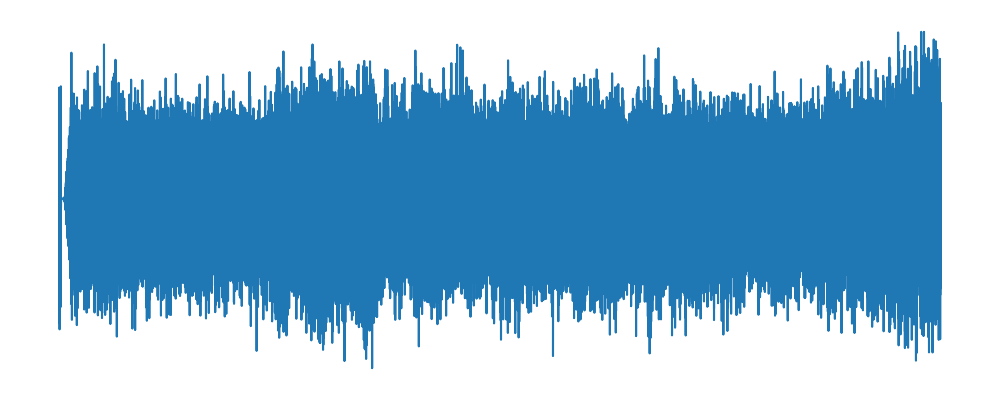
\includegraphics[width=8cm,height=8cm]{waveform.png}};
% \node at (-0.5, 4.5, 0) {\textbf{Waveform}};

% % Arrow from waveform to spec
% \draw[->, thick] (waveform.east) -- (temp.west) node[midway,above] {FFT};


\node[canvas is zy plane at x=0] (temp) at (-1,0,0) {\includegraphics[width=8cm,height=7cm]{spec.png}};
% \node at (-1, 4.5, 0) {\textbf{\\ ~~ Mel-Spectrogram \\}};

% Stem
\pic[shift={(0,0,0)}] at (0,0,0) {RightBandedBox={name=stem,caption=,
        xlabel={{"32"}},zlabel=I/2,fill=\ConvColor,bandfill=\ConvReluColor,%
        height=35,width={2},depth=35}};
% \node at (1, 2, 0) {Stem Conv (3x3)};

% Stage 2
\pic[shift={(1,0,0)}] at (stem-east) {RightBandedBox={name=s2,caption=,
        xlabel={{"16"}},zlabel=I/2,fill=\MBConvColor,bandfill=\ConvReluColor,%
        height=35,width={2},depth=35}};
% \node at (3, 2, 0) {MBConv1 (k3x3)};

% Stage 3
\pic[shift={(1,0,0)}] at (s2-east) {RightBandedBox={name=s3,caption=,
        xlabel={{"24","24"}},zlabel=I/4,fill=\MBConvColor,bandfill=\ConvReluColor,%
        height=30,width={2,2},depth=30}};
% \node at (5.5, 2, 0) {MBConv6 (k3x3) x2};

% Stage 4
\pic[shift={(1.5,0,0)}] at (s3-east) {RightBandedBox={name=s4,caption=,
        xlabel={{"40","40"}},zlabel=I/8,fill=\MBConvColor,bandfill=\ConvReluColor,%
        height=25,width={3,3},depth=25}};
% \node at (8, 2, 0) {MBConv6 (k5x5) x2};

% Stage 5
\pic[shift={(1.5,0,0)}] at (s4-east) {RightBandedBox={name=s5,caption=,
        xlabel={{"80","80","80"}},zlabel=I/16,fill=\MBConvColor,bandfill=\ConvReluColor,%
        height=20,width={4,4,4},depth=20}};
% \node at (11, 2, 0) {MBConv6 (k3x3) x3};

% Stage 6
\pic[shift={(2,0,0)}] at (s5-east) {RightBandedBox={name=s6,caption=,
        xlabel={{"112","112","112"}},zlabel=I/16,fill=\MBConvColor,bandfill=\ConvReluColor,%
        height=20,width={5,5,5},depth=20}};
% \node at (14.5, 2, 0) {MBConv6 (k5x5) x3};

% Stage 7
\pic[shift={(2,0,0)}] at (s6-east) {RightBandedBox={name=s7,caption=,
        xlabel={{"192","192","192","192"}},zlabel=I/32,fill=\MBConvColor,bandfill=\ConvReluColor,%
        height=15,width={6,6,6,6},depth=15}};
% \node at (18.5, 2, 0) {MBConv6 (k5x5) x4};

% Stage 8
\pic[shift={(2.5,0,0)}] at (s7-east) {RightBandedBox={name=s8,caption=,
        xlabel={{"320"}},zlabel=I/32,fill=\MBConvColor,bandfill=\ConvReluColor,%
        height=15,width={7},depth=15}};
% \node at (22, 2, 0) {MBConv6 (k3x3) x1};
        
% Head
\pic[shift={(1,0,0)}] at (s8-east) {RightBandedBox={name=head_conv,caption=,
        xlabel={{"1280"}},zlabel=I/32,fill=\ConvColor,bandfill=\ConvReluColor,%
        height=15,width={10},depth=15}};
% \node at (25.5, 2, 0) {Head Conv (1x1)};

\pic[shift={(1,0,0)}] at (head_conv-east) {Box={name=pool,caption=,
        fill=\PoolColor,opacity=0.5,height=15,width=1,depth=15}};
% \node at (27, 2, 0) {AvgPool};

\pic[shift={(0.5,0,0)}] at (pool-east) {Box={name=fc,caption=,
        xlabel={{"31"}},fill=\ConvColor,%
        height=10,width=2,depth=10}};
% \node at (28, 2, 0) {FC};
        % 
\pic[shift={(0.5,0,0)}] at (fc-east) {Box={name=softmax,caption=,
        xlabel={{"31"}},fill=\SoftmaxColor,%
        height=10,width=2,depth=10,zlabel=I}}; 
% \node at (29.5, 2, 0) {Softmax};

% \node[canvas is zy plane at x=0, right=5cm of softmax-east] (output) {\includegraphics[width=10cm,height=0cm]{DJI_Tello.png}};

% \node[canvas is zy plane at x=0, right=5cm of softmax-east] (output) {\includegraphics[width=10cm,height=0cm]{DJI_Tello.png}};
% Output Node
% \node[canvas is zy plane at x=-3] (drone) at (37.5,0,0) {\includegraphics[width=11cm,height=8cm]{DJI_Tello.png}};
% \node at (37.5, 4.5, 0) {\textbf{Final Classification}};
%%%%%%%%%%%%%%%%%%%%%%%%%%%%%%%%%%%%%%%%%%%%%%%%%%%%%%%%%%%%%%%%%%%%%%%%%%%%%%%%%%%%%%%%
%% Draw connections
%%%%%%%%%%%%%%%%%%%%%%%%%%%%%%%%%%%%%%%%%%%%%%%%%%%%%%%%%%%%%%%%%%%%%%%%%%%%%%%%%%%%%%%%
\draw [connection]  (stem-east)    -- node {\midarrow} (s2-west);
\draw [connection]  (s2-east)    -- node {\midarrow} (s3-west);
\draw [connection]  (s3-east)    -- node {\midarrow} (s4-west);
\draw [connection]  (s4-east)    -- node {\midarrow} (s5-west);
\draw [connection]  (s5-east)    -- node {\midarrow} (s6-west);
\draw [connection]  (s6-east)    -- node {\midarrow} (s7-west);
\draw [connection]  (s7-east)    -- node {\midarrow} (s8-west);
\draw [connection]  (s8-east)    -- node {\midarrow} (head_conv-west);
\draw [connection]  (head_conv-east) -- node {\midarrow} (pool-west);
\draw [connection]  (pool-east) -- node {\midarrow} (fc-west);
\draw [connection]  (fc-east) -- node {\midarrow} (softmax-west);

\end{tikzpicture}
\end{document}
